% ------------------------------------------------------------------------
%                                Capítulo 2
% ------------------------------------------------------------------------
\chapter{Detección de rayos cósmicos}
%\chapter{Marco teórico}
% ------------------------------------------------------------------------
%%Esta sección tiene como propósito presentar la información necesaria para contextualizar el proyecto y revisar el estado del arte.

\section{Rayos Cósmicos}
Los rayos cósmicos primarios son partículas procedentes del espacio cuya energía se debe a su gran velocidad.
Éstas son principalmente nucleos atómicos, fotones y partículas neutras.

Cuando los rayos cósmicos primarios interactúan con la atmósfera terrestre desencadenan un proceso estocástico conocido como lluvia atmosférica extendida (EAS, por sus siglas en inglés).
Esta consiste en una cascada de partículas secundarias (radiación electromagnética de muones y electrones) que se dirigen hacia la superficie de la Tierra a altas velocidades en la dirección del rayo cósmico incidente ~\citep{ASOREY2012}.
Esta cascada es producida por la interacción de un rayo cósmico primario con átomos de la parte superior de la atmósfera.

%La lluvia atmosférica extendida es una cascada de radiación electromagnética de muones y nucleones producida por la interacción de un rayo cósmico primario con atomos de la parte superior de la atmósfera. En la Figura~\ref{lluvia} se observa como las EAS son detectadas a nivel del suelo mediante arreglos de detectores Cherenkov de agua.

Actualmente se utilizan dos tipos de métodos para la detección de rayos cósmicos: los métodos indirectos y los directos.
En los métodos directos las partículas primarias inciden directamente con el detector, por lo cual los dispositivos de detección se encuentran situados en satélites, globos o aviones.
Los métodos indirectos detectan la cascada de partículas secundarias producida por la interacción con la atmósfera.
Para la detección de éstas se  utilizan detectores ubicados en tierra como WCD, telescopios de fluorescencia y detectores de centelleo ~\citep{schlaepfer2003cosmic}.
En la Figura~\ref{lluvia} se observa como las EAS pueden ser detectadas a nivel del suelo mediante arreglos de detectores Cherenkov de agua.

\begin{figure}[H]
\centering
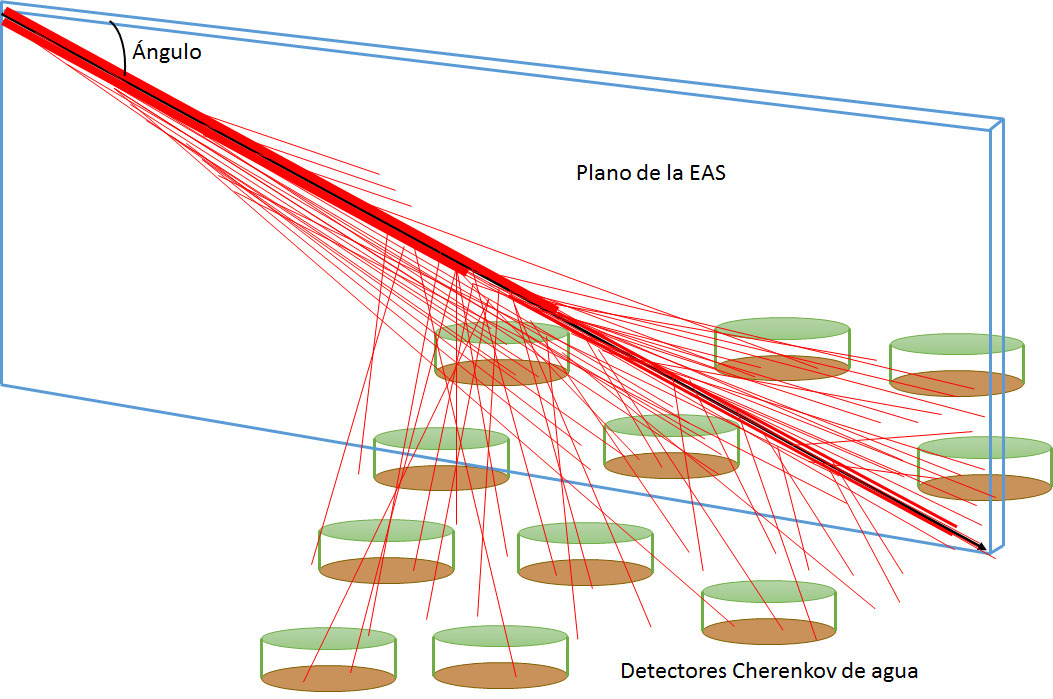
\includegraphics[width=0.8\textwidth]{Figs/imagenllu.jpeg} 
\caption[Lluvia atmósferica extendida (EAS)]
{Lluvia atmósferica extendida (EAS) detectada mediante un arreglo de varios WCD.
Procesando el tiempo con el cual el evento llega a cada detector de superficie se determina el ángulo de incidencia de las partículas ~\citep{hernandez2018procedimiento}.}
\label{lluvia}
\end{figure}

\section{Proyecto LAGO}
El proyecto LAGO (por sus siglas en inglés, \textit{The Latin American Gian Observatory}) es un observatorio de astropartículas que se dedica al estudio de temas relacionados con astrofísica y clima espacial y que cuenta con equipos instalados en diferentes países de América Latina.

\subsection{Detectores WCD de LAGO}
El proyecto LAGO utiliza tanques de agua como detectores de partículas.
Un WCD típico de LAGO es un tanque lleno de agua purificada cuyo volumen oscila entre 1~$m^3$ y 40~$m^3$.
En su interior tiene una bolsa hecha por un tejido altamente difusivo y reflectante de Tyvek~\textregistered1073D para contener todo el volumen de agua y aumentar la eficiencia de detección.
El objetivo de este recubrimiento es difundir los fotones Cherenkov captados por los tubos fotomultiplicadores (PMT, por sus siglas en inglés) y reducir la dependencia de la señal de la trayectoria de las partículas secundarias dentro del detector, ya que con esto los fotones se distribuirán uniformemente dentro del tanque (Ver Figura~\ref{tank}).

\begin{figure}[H]
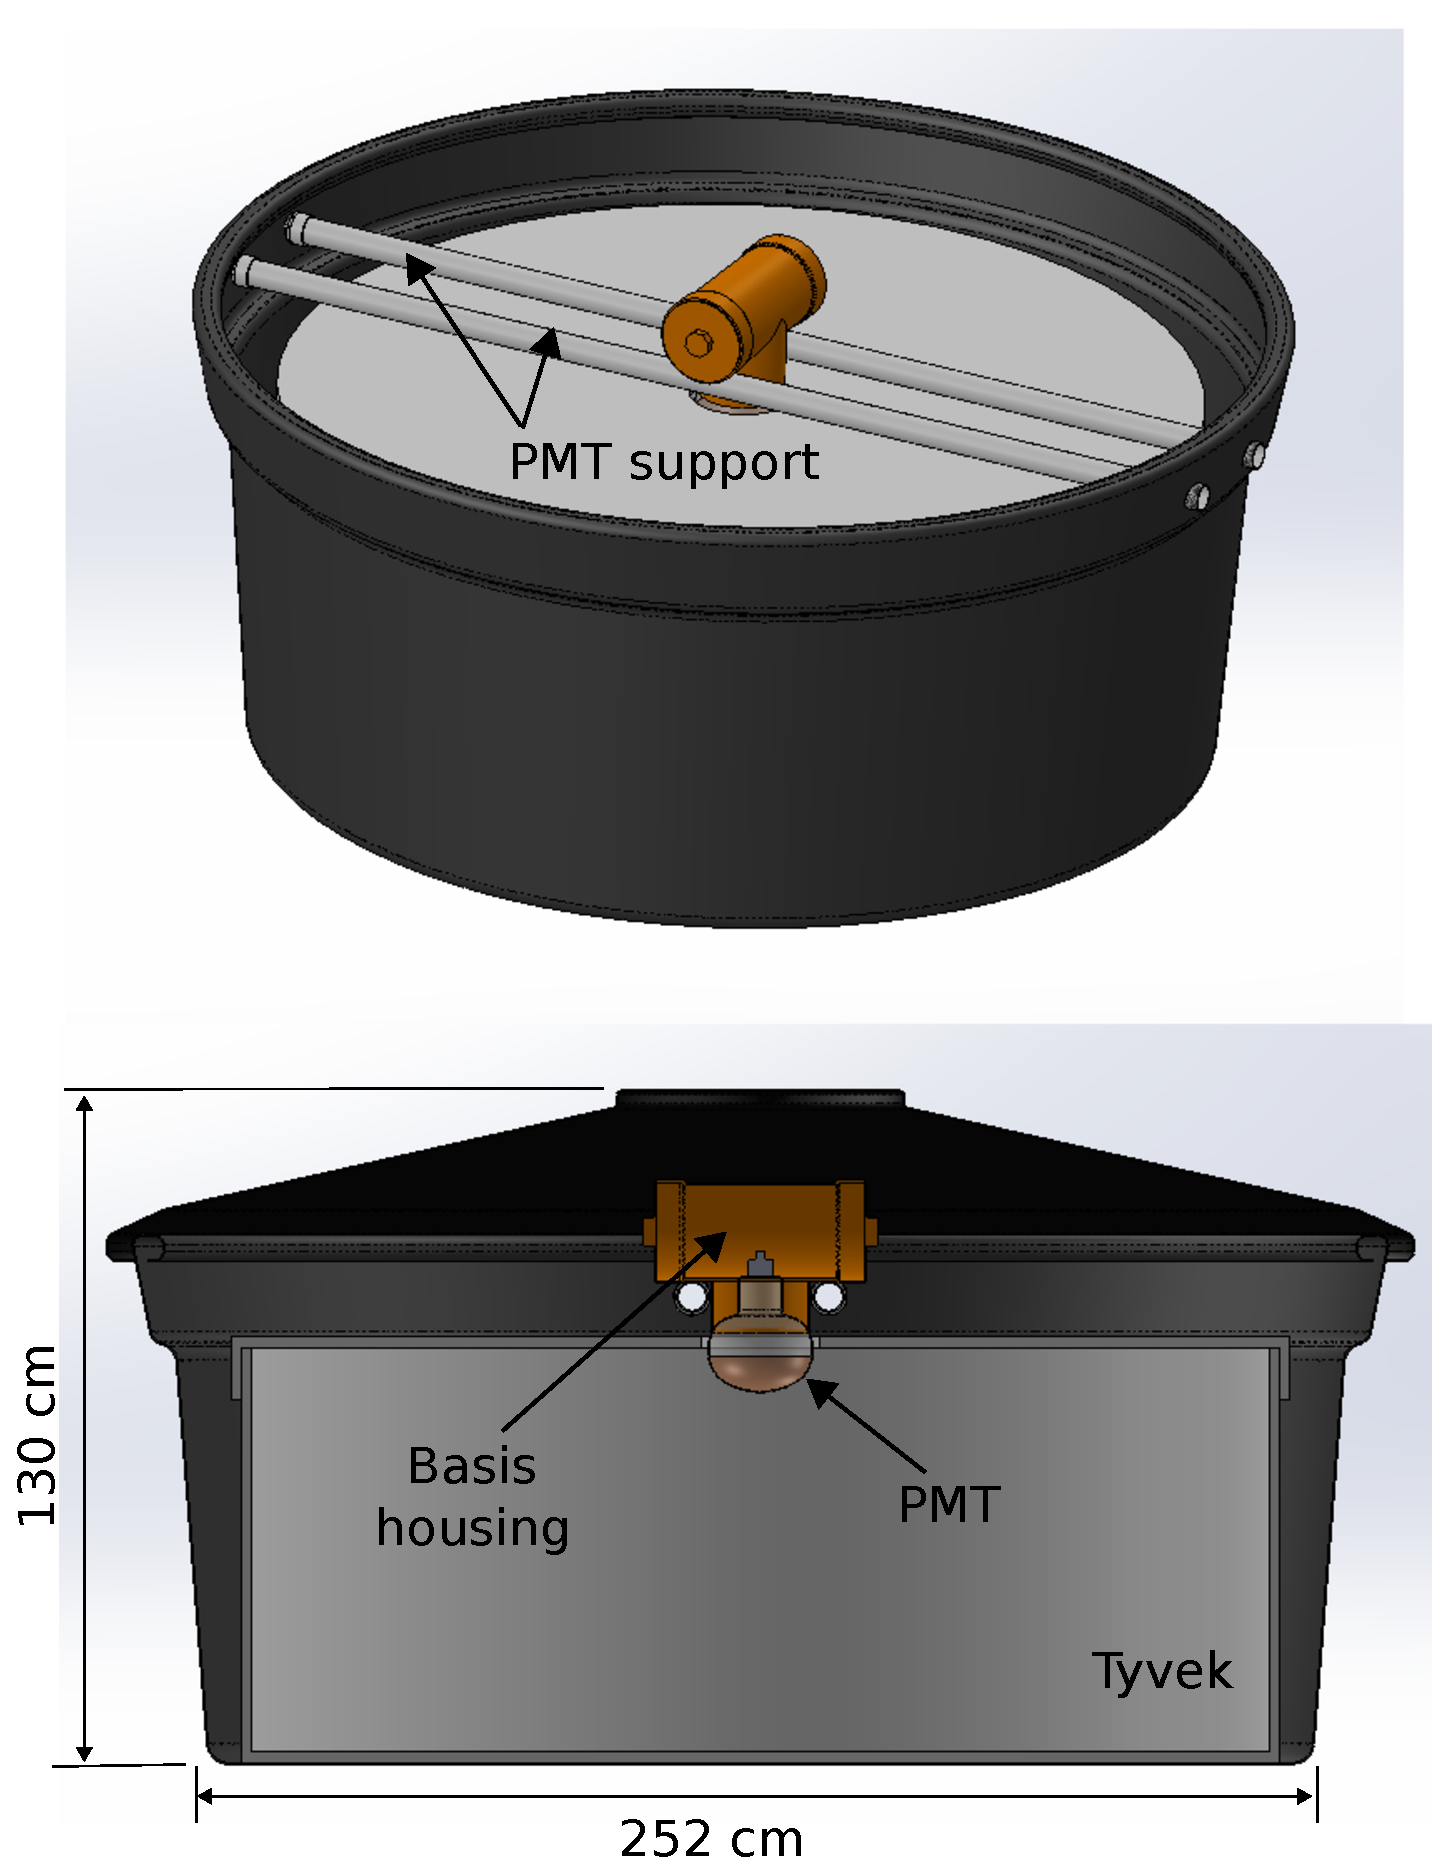
\includegraphics[scale=0.4]{Figs/Tank.eps} 
\centering
\caption[Ilustración de un Detector Cherenkov]{.~\citep{hernandez2018procedimiento}}
\label{tank}
\end{figure}

\subsection{Tubo fotomultiplicador}
Los PMT son los dispositivos fotosensores más empleados debido tanto a su gran versatilidad como sus características (respuesta rápida, alta sensibilidad y alto factor de ganancia).
Un tubo fotomultiplicador funciona como transductor y a su vez como amplificador, es decir, que a partir de una luz detectada se produce una corriente eléctrica fácilmente medible.

En la Figura~\ref{foto} se muestra el funcionamiento interno de un PMT.
Cuando los fotones de luz visible alcanzan el fotocátodo, éste emite fotoelectrones de baja energía.
Estos electrones son acelerados y multiplicados en campos eléctricos secuenciales aplicados entre los electrodos del PMT llamados dínodos.
En los dínodos la señal eléctrica es suficientemente grande para poder ser manejada con amplificadores y analizadores de pulsos convencionales.~\citep{kaptanoglu2018characterization}.


LAGO utiliza tubos fotomultiplicadores PMT Hamamatsu R5912 de 8 pulgadas desarrollados por Hamamatsu Photonics los cuales se encuentran ubicados sobre el volumen de agua donde inciden los fotones de Cherenkov. 
Estos PMT tienen 10 etapas enfocadas linealmente y su circuito de alimentación está constituido por un divisor de voltaje, una fuente de alimentación de alto voltaje y un preamplificador para acondicionar las amplitudes de los pulsos de salida.
La tensión de polarización del PMT está en el rango de 0~V a 2000~V respecto a tierra y puede controlarse con una baja tensión en el rango de 0~V a 5~V.

\begin{figure}[H]
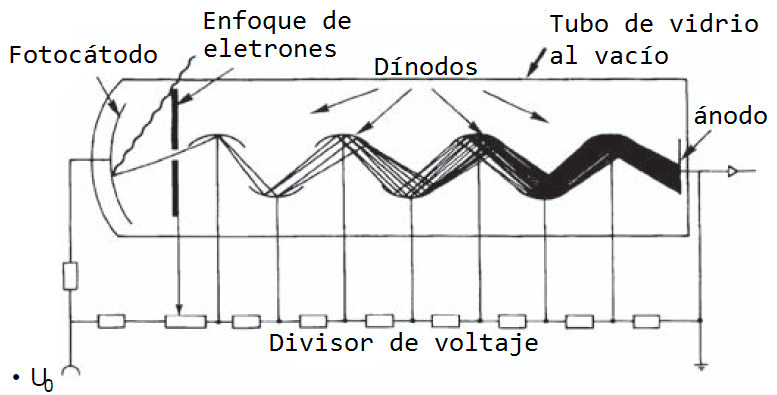
\includegraphics[scale=0.35]{Figs/pmtll.jpeg} 
\centering
\caption[Esquema de funcionamiento de un fotomultiplicador]{Esquema de funcionamiento de un fotomultiplicador.
El fotocátodo convierte la energía de luz incidente en una corriente de electrones por efecto fotoeléctrico.
El campo eléctrico creado entre los dínodos permite acelerar y guiar los electrones a lo largo del multiplicador.
El divisor de voltaje está compuesto por un arreglo de resistencias que dividen el voltaje y alimentan los dínodos.~\citep{hernandez2018procedimiento}}
\label{foto}
\end{figure}

El sistema de adquisición implementado por LAGO permite suministrar las tensiones requeridas en la base de PMT.
Un detector de WCD normalmente emite pulsos con un tiempo de subida de $\sim$10~ns y un tiempo de bajada de $\sim$70~ns.
La forma de los pulsos que vienen del detector dependen de la pureza del agua, la reflectividad del material de difusión y la geometría del tanque.~\citep{haro2016data}.
En la Figura~\ref{detec} se muestra el sistema de adquisición implementado en uno de los detectores instalado en la UIS, mientras que en la Figura~\ref{sistema_adquisicion} se muestra el diagrama de bloques de un detector WCD de LAGO.

\begin{figure}[H]
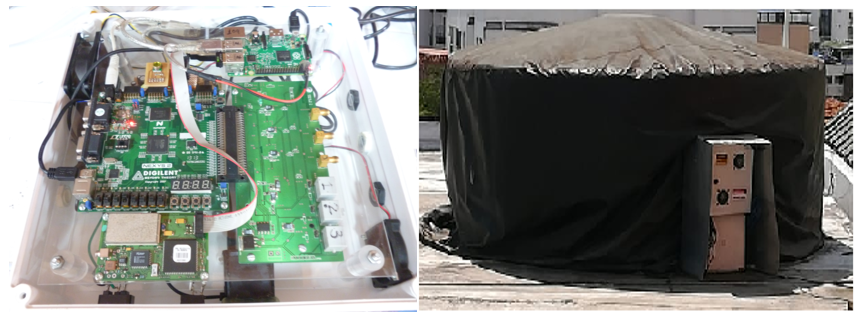
\includegraphics[scale=0.6]{Figs/lagoelectro.PNG} 
\centering
\caption[Sistema de adquisición LAGO original]{Sistema de adquisición LAGO original.
A la derecha: WCD Chitagá ubicado en el campus central de la Universidad Industrial de Santander en Bucaramanga en Santander, Colombia.
A la izquierda: electrónica del sistema de adquisición del detector.}
\label{detec}
\end{figure}

\begin{figure}[H]
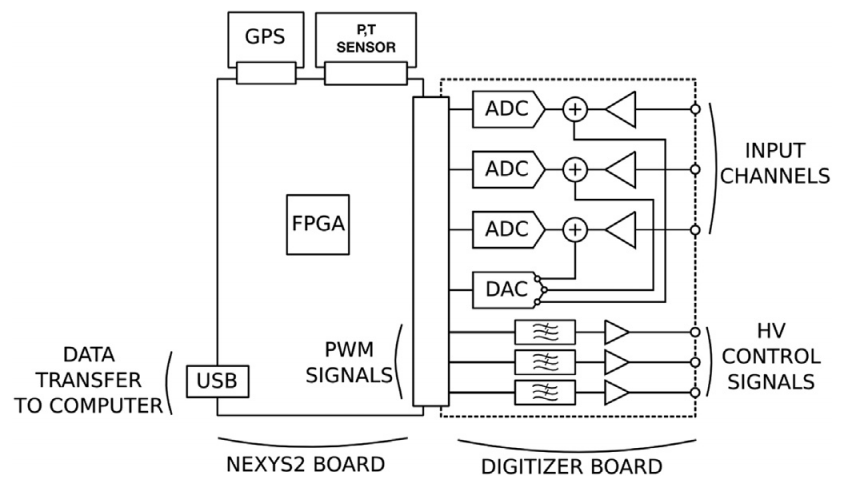
\includegraphics[scale=0.6]{Figs/bloquelago.PNG} 
\centering
\caption[Componentes principales del sistema de adquisición]{Componentes principales del sistema de adquisición: tarjeta digitalizadora de tres canales, placa Nexys-II y periféricos (GPS y sensores de temperatura y presión).~\citep{haro2016data}}.
\label{sistema_adquisicion}
\end{figure}


